% !TEX program = lualatex
\documentclass[10pt, leqno]{ltjsarticle} % 日本語をそのまま扱えるクラス
% \usepackage[margin=28mm]{geometry}
\usepackage{amsmath,amssymb,mathtools}
\usepackage{amsthm}
\usepackage{tikz}
\usetikzlibrary{arrows.meta,positioning,calc}

\usepackage[
  top=15mm,     % 上余白
  bottom=15mm,  % 下余白
  left=10mm,    % 左余白
  right=10mm,    % 右余白
  landscape,
  margin=10mm
]{geometry}
% \usepackage[landscape,margin=20mm]{geometry} % 余白はお好みで
\usepackage{paracol}
\columnratio{0.5,0.5}             % 左右を 1:1 に
\setlength{\columnseprule}{0.4pt} % 真ん中の縦線

% ---- 記号・マクロ ----
\newcommand{\xto}{\mathrel{\xrightarrow{}}}
\newcommand{\into}{\hookrightarrow}
\newcommand{\epi}{\twoheadrightarrow}
\newcommand{\pto}{\rightrightarrows}
\newcommand{\cls}[1]{\bigl(#1\bigr)}
\newcommand{\redjoin}{\wedge}
\newcommand{\shrink}{\phi}
\newcommand{\Ex}{E}        % suspension functor E
\newcommand{\Ox}{\Omega}   % loop functor Omega
\newcommand{\id}{\mathrm{id}}
% --- Toda bracket helpers ---
\newcommand{\toda}[1]{\{\,#1\,\}}              % {a,b,c}
\newcommand{\todai}[2][]{\{\,#2\,\}_{#1}}      % {a,b,c}_i   (#1 は添字, 空なら無し) 
\newcommand{\gen}[1]{\{\,#1\,\}}       % ⟨generator⟩ 表記を { } で統一
\newcommand{\Ker}{\operatorname{Ker}}
\newcommand{\im}{\operatorname{Im}}
\newcommand{\hs}[2]{\bigl[#1,#2\bigr]}   % 一般のホモトピー集合
\newcommand{\pis}[2]{\pi_{#1}(#2)}       % 左が球面のときのホモトピー群
\newcommand{\ext}[1]{\overline{#1}}     % extension
\newcommand{\coext}[1]{\widetilde{#1}}  % coextension
\newcommand{\z}{\mathbb{Z}}

% ---- theorem-like environments ----
\numberwithin{equation}{section}
\theoremstyle{plain}
\newtheorem{theorem}{Theorem}[section]
\newtheorem{lemma}[theorem]{Lemma}
\newtheorem{proposition}[theorem]{Proposition}
\newtheorem{corollary}[theorem]{Corollary}
\theoremstyle{definition}
\newtheorem{definition}[theorem]{Definition}
\newtheorem{example}[theorem]{Example}
\newtheorem{notation}[theorem]{Notation}
\newtheorem{assumption}[theorem]{Assumption}
\theoremstyle{remark}
\newtheorem{remark}[]{Remark}

% \title{PART 1 \quad CHAPTER I\\[2mm] General Composition and Secondary Composition}
\author{}
\date{}

\begin{document}

% --- CHAPTER II ---
\setcounter{section}{1}
\section{Generalized Hopf Invariant and Secondary Composition}

\begin{paracol}{2}

以下では, 球面の homotopy 群
\[
\pis{p}{S^m} \quad(=\hs{S^p}{S^m})
\]
について考察を進める. \\
$\iota_n\in\pis{n}{S^n}$ を $S^n$ の恒等写像の homotopy クラスとする. \\
明らかに, 
$\iota_n\circ\alpha=\alpha=\alpha\circ\iota_p$ ($\alpha\in\pis{p}{S^m}$) である. \\
(1.7) から次が従う：
\begin{equation}\label{eq:2.1}
% (2.1).\
\raisetag{3ex}
\begin{aligned}[t]
\alpha\circ(\beta_1\pm\beta_2)
&=\alpha\circ\beta_1\ \pm\ \alpha\circ\beta_2,\\
(\alpha_1\pm\alpha_2)\circ E\beta
&=\alpha_1\circ E\beta\ \pm\ \alpha_2\circ E\beta,
\end{aligned}
\end{equation}
特に, 任意の整数 $k$ に対して,
\[
k(\alpha\circ\beta)=\alpha\circ(k\beta),\qquad
k(\alpha\circ E\beta)=(k\alpha)\circ E\beta
\]
が成り立つ. \\
$\alpha\in\pis{p}{S^m}$ と $\beta\in\pis{q}{S^n}$ の \emph{reduced join}
\[
\alpha\ \redjoin\ \beta\ \in\ \pis{p+q}{S^{m+n}}
\]
は, 第1章で導入した (1.3) の特別な写像 
$\phi_{p,q}$ と $\phi_{m,n}$ を用いて定義される. \\
特に, $E^n$ の定義から次が成り立つ. 
\[
E^n\alpha=\alpha\ \redjoin\ \iota_n
\]
また \emph{secondary composition}
\[
\todai[n]{\alpha,\ E^n\beta,\ E^n\gamma}
\in\pi_{i+n+1}(S^m) / 
(\alpha\circ E^n\pi_{i+1}(S^k) + \pi_{j+n+1}(S^m)\circ E^{n+1}\gamma)
\]
は, 
\[
\alpha\in\pis{k+n}{S^m},\qquad
\beta\in\pis{j}{S^k},\qquad
\gamma\in\pis{i}{S^j}
\]
が, (1.13) の条件が満たされるときに定義される. \\
ここでは (1.14) の $d$ の代わりに, (1.8) に現れる写像 $d_{i+n}$ を用いる. \\
もちろん, 第1章での議論はこの特別な場合にもそのまま適用できる. 

\switchcolumn

\noindent
\textbf{(1.7).}\
\(f:Y\to Z,\ g:W\to X \text{ に対して, 次は準同型である.}\)\\
\(
f_*:[EX, Y] \to [EX,Z],\quad Eg^*:[EX,Y]\to[EW,Y].
\)

\noindent
$n\ge 0$ を整数とし, 
$\alpha\in[\Ex^n Y, Z]$, $\beta\in[X, Y]$, $\gamma\in[W, X]$ に対して,\\
\textbf{(1.13).}\
\(\alpha\circ \Ex^n\beta=0,\ \beta\circ \gamma=0\).

\noindent
\textbf{(1.14).}\ $H:\ (\Ex^{n+1}W,w_0)\to (Z,z_0)$ を, 次で定める. \\
\(
H(d(w,t))=
\begin{cases}
a\bigl(\Ex^n B_{2t-1}(w)\bigr), & \tfrac12\le t\le 1,\\[2mm]
A_{1-2t}\bigl(\Ex^n c(w)\bigr), & 0\le t\le \tfrac12.
\end{cases}
\)

\noindent
\textbf{(1.8).}\
\(d_n:S^n\times I\longrightarrow S^{n+1},\quad
d_n\bigl(\psi_n(t_1,\ldots,t_n),t\bigr)=\psi_{n+1}(t_1,\ldots,t_n,t).\)


\end{paracol}

\begin{paracol}{2}

次に, [9] に従って $S^m$ の \emph{reduced product} の概念を導入し, 
必要な結果を述べる. \\
$(S^m)_\infty$ を $S^m$ の reduced product と記す. \\
$(S^m)_\infty$ は, 単位 $e_0$ を持つ自由半群であり, 
その生成元の集合は $S^m-e_0$ である. \\
$(S^m)_\infty$ の各点は, 
$x_1\cdots x_t$ ($x_1,\ldots,x_t\in S^m$) という積で表される. \\
正の整数 $t$ を固定するとき, $(S^m)_t$ はそのような積の集合を表す. 
%  (次ページへ続く) 

\switchcolumn

\noindent
\cite{James1955}
I.~M.~James,
\newblock Reduced product spaces,
\newblock Ann. of Math., {\bf 62} (1955), 170--197.
  
\end{paracol}

\begin{paracol}{2}

$(S^m)_t$ の位相は,
積空間 $S^m\times\cdots\times S^m$ ($t$ 回) 
からの等化写像
\[
S^m\times\cdots\times S^m \ \longrightarrow\ (S^m)_t,\qquad
(x_1,\ldots,x_t)\ \longmapsto\ x_1\cdots x_t
\]
のもとで与える. 
$(S^m)_t-(S^m)_{t-1}$ は開な $tm$-cell になる .\\ 
弱位相を入れると, $(S^m)_\infty$ は CW-complex であり, 
$(S^m)_t$ はその $tm$-skeleton になる. \\
自然な方法で $(S^m)_1$ を $S^m$ と同一視する. 

$f:(S^q,e_0)\to(S^m,e_0)$ に対して, 写像
\[
(f)_t:\ (S^q)_t\longrightarrow(S^m)_t,\qquad (t=1,2,\ldots,\infty)
\]
を
\[
(f)_t(y_1\ldots y_t):=f(y_1)\ldots f(y_t)
\]
で定める. 明らかに $s\le t$ ならば $(f)_s=(f)_t\ |_{(S^q)_s}$ が成り立つ. 

標準的な埋め込み $i:S^m\into\Omega S^{m+1}$ は,
次のように, 
$(S^m)_\infty$ 全体に拡張される. \\
$x_1\cdots x_t\in S^{m+1}$ 
に対して, 
\(t\) 個の loop $i(x_1),\ldots,i(x_t)$ の適切に重み付けした和で表される\\
\(S^{m+1}\) の loop を対応させる.
得られる写像は単射であり, 
\[
i:\ (S^m)_\infty\longrightarrow\Omega S^{m+1}
\]
と書き, これも「標準 (canonical) 埋め込み」と呼ぶ. 

次の図式は homotopy 的に可換である：
\begin{equation}\label{eq:2.2}
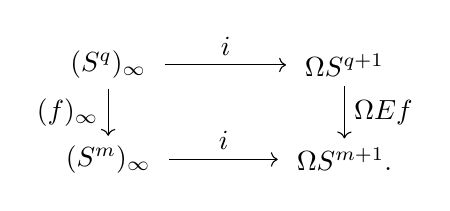
\begin{tikzpicture}[baseline=(current bounding box.center)]
  \node (A) at (0,1.2) {$\ (S^q)_\infty\ $};
  \node (B) at (3,1.2) {$\ \Omega S^{q+1}\ $};
  \node (C) at (0,0)   {$\ (S^m)_\infty\ $};
  \node (D) at (3,0)   {$\ \Omega S^{m+1}.\ $};
  \draw[->] (A) -- node[above] {$i$} (B);
  \draw[->] (C) -- node[above] {$i$} (D);
  \draw[->] (A) -- node[left] {$(f)_\infty$} (C);
  \draw[->] (B) -- node[right] {$\Omega Ef$} (D);
\end{tikzpicture}
\tag{2.2}
\end{equation}

reduced product に関する主結果の一つとして, \\
標準埋め込みは homotopy 群の同型を誘導する：
\[
i_*:\ \pi_q\bigl((S^m)_\infty\bigr)\ \xrightarrow{\;\cong\;}\ 
\pi_q\bigl(\Omega S^{m+1}\bigr),\qquad(\forall\,q).
\]
したがって, 
$(S^m)_\infty$ と $\Omega S^{m+1}$ は同じ singular homotopy type を持ち, 
ゆえに次を得る. 

\begin{lemma}\label{lemma:2.1}
任意の有限 \textnormal{cell complex (より一般には CW-complex)} $K$ に対して,
\[
i_*:\ [K, (S^m)_\infty]\ \longrightarrow\
[K, \Omega S^{m+1}]
\]
は全単射である. 
\end{lemma}

\end{paracol}

\begin{paracol}{2}

全単射 $\Omega_1$ を, 次で定める：
\begin{equation}\label{eq:2.3}
\Omega_1\ :=\ i_*^{-1}\circ \Omega_0:\ 
[EK, S^{m+1}] \xrightarrow{}\ 
[K, (S^m)_\infty].
\tag{2.3}
\end{equation}
特に, すべての $k$ に対して,
\[
\Omega_1:\ \pi_{k+1}(S^{m+1})\ 
\xrightarrow{\cong}\ \pi_k\bigl((S^m)_\infty\bigr).
\]

\switchcolumn

\noindent
\textbf{(1.10).}\
\(\Omega_0: [EX, Y]\xrightarrow{\cong} [X, \Omega Y].\)
  
\end{paracol}

\begin{paracol}{2}


包含 $i':S^m\into(S^m)_\infty$ に対して, 次の図式は可換である：
\begin{equation}\label{eq:2.4}
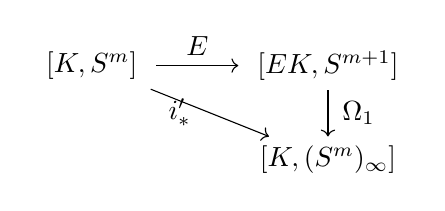
\begin{tikzpicture}[baseline=(current bounding box.center)]
  \node (A) at (0,1.2) {$\ [K, S^m]\ $};
  \node (B) at (3,1.2) {$\ [EK, S^{m+1}]\ $};
  \node (C) at (3,0)   {$\ [K, (S^m)_\infty]\ $};
  \draw[->] (A) -- node[above] {$E$} (B);
  \draw[->] (A) -- node[left] {$i'_*\,\,$} (C);
  \draw[->] (B) -- node[right] {$\,\Omega_1$} (C);
\end{tikzpicture}
\tag{2.4}
\end{equation}

写像 \(h'_m\) を, 次で定める.
\[
h'_m:\ \bigl((S^m)_2, S^m\bigr)\ \to\ (S^{2m},e_0),
\]
\[
h'_m(xy)=\phi_{m,m}(x,y)\qquad(x,y\in S^m).
\]
さらに,
\begin{equation}\label{eq:2.5}
h_m:\ \bigl((S^m)_\infty,\ S^m\bigr)\ \longrightarrow\
\bigl((S^{2m})_\infty,\ e_0\bigr)
\tag{2.5}
\end{equation}
を [9] で定義された \(h'_m\) の combinatorial extension とする. \\
このとき, 次の図式は可換である：
\begin{equation}\label{eq:2.6}
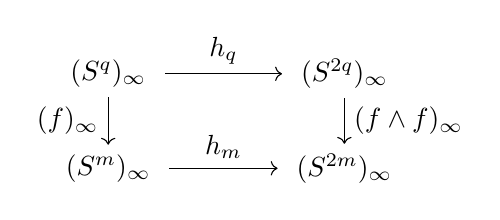
\begin{tikzpicture}[baseline=(current bounding box.center)]
  \node (A) at (0,1.2) {$\ (S^q)_\infty\ $};
  \node (B) at (3,1.2) {$\ (S^{2q})_\infty\ $};
  \node (C) at (0,0)   {$\ (S^m)_\infty\ $};
  \node (D) at (3,0)   {$\ (S^{2m})_\infty\ $};
  \draw[->] (A) -- node[above] {$h_q$} (B);
  \draw[->] (C) -- node[above] {$h_m$} (D);
  \draw[->] (A) -- node[left] {$(f)_\infty$} (C);
  \draw[->] (B) -- node[right] {$(f\wedge f)_\infty$} (D);
\end{tikzpicture}
\tag{2.6}
\end{equation}

一般に, 写像
\(
h':\ \bigl((S^m)_k,\ (S^m)_{k-1}\bigr)\ \longrightarrow\ (S^{km},e_0)
\)
の combinatorial extension,
\[
h:\ (S^m)_\infty\ \longrightarrow\ (S^{km})_\infty
\]
は, 次式で定義される：
\[
h(x_1\ldots x_t)\ 
:=\ \prod_{\sigma}\ h'\!\bigl(x_{\sigma(1)}\cdots x_{\sigma(k)}\bigr),
\]
ここで, $\sigma$ は, 
$\{1,2,\ldots,k\}$ を, $\{1,2,\ldots,t\}$ へ, 
単調増加に移す写像であり,\\ 
$(S^{km})_\infty$ における積 
$\prod\nolimits_{\sigma}$ 
の順序は右 (あるいは左) からの辞書式順序とする. 

次に, \emph{generalized Hopf invariant} $H$ を,
\begin{equation}\label{eq:2.7}
H\ :=\ \Omega_1^{-1}\circ h_{m*}\circ \Omega_1:\ 
[EK, S^{m+1}]\ \longrightarrow\ [EK, S^{2m+1}]
\tag{2.7}
\end{equation}
で定める. 
特に, すべての $i$ について準同型,
\[
H:\ \pi_{i+1}(S^{m+1})\ \longrightarrow\ \pi_{i+1}(S^{2m+1})
\]
を得る. 

\begin{proposition}\label{prop:2.2}
% Prop2.2.\
$K,L$ を有限 cell complex とする. \\
$\alpha\in[EK, S^{m+1}], \ \beta\in[L,K], \ \gamma\in\pi_r(S^r)$ 
に対して, 次が成り立つ：\\
\[
H(\alpha\circ E\beta)\ =\ H(\alpha)\circ E\beta,
\]
\[
H(E\gamma\circ\alpha)\ =\ E(\gamma\wedge\gamma)\circ H(\alpha).
\]
\end{proposition}

  
\end{paracol}


\begin{paracol}{2}

\noindent
\textbf{Proof.}\
\begin{align*}
H(\alpha\circ E\beta) 
& = (\Omega_0^{-1}\circ i_{*}\circ h_{m*}\circ i_{*}^{-1}\circ \Omega_0)(\alpha\circ E\beta)
&& \text{by (2.7)},\\
& = \Omega_0^{-1}\!\bigl((i_*\circ h_{m*}\circ i_*^{-1})(\Omega_0\alpha)\bigr)\circ E\beta
&& \text{by (1.12)},\\
& = (\Omega_0^{-1}\circ i_*\circ h_{m*}\circ i_{*}^{-1}\circ\Omega_0)(\alpha)\circ E\beta
&& \text{by (1.12)},\\
& = H(\alpha)\circ E\beta .
\end{align*}

\switchcolumn

\noindent
\textbf{(1.12).}\
\(\Omega_0(\beta\circ E\alpha) = \Omega_0\beta\circ\alpha,\qquad
\Omega_0(\gamma\circ\beta) = \Omega\gamma \circ \Omega_0\beta .\)
  
\end{paracol}

\begin{paracol}{2}

次に,
\[
H(E\gamma\circ\alpha)
= \Omega_0^{-1}\!\bigl((i_*\circ h_{m*}\circ i_*^{-1})(\Omega E\gamma)\bigr)\circ \Omega_0(\alpha)
\]
に対し, 図式 (2.6) と (2.2) , および (1.12) を用いると
\[
\Omega_1^{-1}\!\bigl(\Omega^{-1}E(\gamma\wedge\iota_m)\bigr)\circ (\Omega_1^{-1}\circ h_{m*}\circ \Omega_1)(\alpha)
= E(\gamma\wedge\gamma)\circ H(\alpha)
\]
を得る. 
\qed

\medskip

\begin{proposition}\label{prop:2.3}
% \noindent
% \textbf{Prop2.3.}\
$n\ge1$ とし, 元
\[
\alpha\in[E^nK, S^{m+1}],\quad
\beta\in[L, K],\quad
\gamma\in[M, L]
\]
が条件
\[
\alpha\circ E^n\beta=0,\qquad \beta\circ\gamma=0
\]
を満たすと仮定する. このとき,
\[
H\!\bigl(\,\{\,\alpha,\ E^n\beta,\ E^n\gamma\,\}_n\bigr)\ \subset\
\{\,H(\alpha),\ E^n\beta,\ E^n\gamma\,\}_n .
\]
\end{proposition}
  
\end{paracol}

\begin{paracol}{2}

\noindent
\textbf{Proof.}\
Prop1.7 より, $\{\,\alpha,E^n\beta,E^n\gamma\,\}_n$ の任意の元は, \\
$\alpha$ の extension $\overline\alpha\in[E^n(K\cup_\beta CL), S^{m+1}]$
と, $\gamma$ の coextension 
$\widetilde\gamma$ の $n$-懸垂 $E^n\tilde\gamma$ を用いて,
\[
(-1)^n\,\overline{\alpha}\circ E^n\widetilde{\gamma}
\]
と書ける. Prop \ref{prop:2.2} により,
\[
H((-1)^n\overline\alpha\circ E^n\widetilde\gamma)
=(-1)^n H(\overline\alpha)\circ E^n\widetilde\gamma .
\]
包含の類 $\iota\in[E^nK, E^n(K\cup_\beta CL)]$ をとると, 
$\iota$ は懸垂元であり $\overline\alpha\circ\iota=\alpha$. 
Prop \ref{prop:2.2} から,
\[
H(\alpha)=H(\overline\alpha\circ\iota)=H(\overline{\alpha})\circ\iota
\]
が従い, $H(\overline\alpha)$ は $H(\alpha)$ の extension である. 
よってProp1.7 を再び用いると,
\[
(-1)^n H(\ext{\alpha})\circ E^n\coext{\gamma}\ \in\
\{\,H(\alpha),\ E^n\beta,\ E^n\gamma\,\}_n
\]
となり, 主張が従う. 
\qed

上の $(S^m)_\infty$ に関する議論および generalized Hopf invariant に関する結果は, \\
$S^m$ を適当な空間 (例えば有限 cell complex) 
で置き換えても成り立つことを付言しておく. 

\switchcolumn

\noindent
\textbf{Prop1.7.}\
\(\todai[n]{\alpha, E^n\beta, E^n\gamma}
= (-1)^n\gen{\overline{\alpha}\circ E^n\widetilde{\gamma}}\).

\noindent
\textbf{Prop2.2.}\
\(H(\alpha\circ E\beta) = H(\alpha)\circ E\beta.\)

\end{paracol}

\begin{paracol}{2}

\begin{theorem}[James {[10]}; Toda {[21]}]\label{thm:2.4}
% Th2.4.\
$p$ を素数, $m>1$ とする. 
連続写像
\[
h:\ ((S^m)_\infty,(S^m)_{p-1})\longrightarrow ((S^{pm})_\infty,e_0)
\]
であって, $e^{pm}$ を $S^{pm}-e_0$ へ同相に移すものをとる. 
\begin{enumerate}
\item $m$ が奇数で $p=2$ のとき, 次は全ての $i$ に対して同型である. 
\[
h_*:\ \pi_i\bigl((S^m)_\infty,S^m\bigr)\ \longrightarrow\ 
\pi_i\bigl((S^{2m})_\infty\bigr).
\]
\item $m$ が偶数のとき, 次は $i<(p+1)m-1$ に対して同型である.
\[
h_*:\ \pi_i\bigl((S^m)_\infty,(S^m)_{p-1}\bigr)\ \longrightarrow\ 
\pi_i\bigl((S^{pm})_\infty\bigr).
\]
さらに, 全ての $i$ に対して $p$-成分についての同型を与える. 
\end{enumerate}
\end{theorem}

\noindent
\textbf{Proof.}\
[6]のTh2 を用いれば, 
\[
h_*:\ \pi_i\bigl((S^m)_\infty,(S^m)_{p-1}\bigr)\ \longrightarrow\ \pi_i\bigl((S^{pm})_\infty\bigr)
\]
が, $i<(p+1)m-1$ に対して同型であることが従う. 

\switchcolumn

\noindent
\cite{James1956}
I.~M.~James,
\newblock Suspension triad of a sphere,
\newblock Ann. of Math., {\bf 63} (1956), 407--429.

\noindent
\cite{Toda1956}
H.~Toda,
\newblock On double suspension $E^2$,
\newblock Jour. of Inst. Poly. Osaka City Univ., {\bf 7} (1956), 103--145.

\noindent
\cite{BlakersMassey1952}
A.~L.~Blakers and W.~S.~Massey,
\newblock The homotopy groups of a triad II,
\newblock Ann. of Math., {\bf 55} (1952), 192--201.\\
\textbf{Th2.}\ \(\pi_i(X,A)=0\ (i<n),\ \pi_i(A)=0\ (i<m),\ 
p:(X,A)\to(X/A,*),\)\\
\(\Longrightarrow p_*:\pis{i}{X,A}\to\pis{i}{X/A}\)
は, \(i<n+m-1\) で同型, \\
\(\pis{i}{S^m_\infty, S^m_{p-1}}=0\ (i<pm),\ 
\pis{i}{S^m_{p-1}} = 0\ (i<m).\)


\end{paracol}

\begin{paracol}{2}


次に, $(S^m)_\infty$ のコホモロジー構造について述べる. \\
これは, $S^m$ の $k$-重積 $S^m\times\cdots\times S^m$ のコホモロジー構造から, \\
$(S^m)^k$ への等化写像を通して計算される. \\
$H^{km}\bigl((S^m)_\infty\bigr)$ の生成元 $u_k$ を, 
$km$-cell $e^{km}$ に双対な元としてとると, 次が成り立つ：\\
$m$ が奇数のとき, 
\[
u_1\,u_{2k}=u_{2k+1},\qquad
u_{2k}\,u_{2h}=\binom{k+h}{k}\,u_{2(k+h)}.
\]
$m$ が偶数のとき, 
\[
u_k\,u_h=\binom{k+h}{k}\,u_{k+h}.
\]
係数体を,
\[
\Lambda=
\begin{cases}
\mathbb{Z}, & m\ \text{奇数かつ } p=2,\\
\mathbb{Z}_p, & m\ \text{偶数}.
\end{cases}
\]
とする. このとき, 次のことが簡単に確かめられる. 
\[
i^*:H^i\bigl((S^m)_\infty;\Lambda\bigr)\to H^i\bigl((S^m)_{p-1};\Lambda\bigr)
\ \ \text{は} \ 
i<pm \ \text{で同型 .}
\]
\[
h^*:H^i\bigl((S^{pm})_\infty;\Lambda\bigr)\to H^i\bigl((S^m)_{\infty};\Lambda\bigr)
\ \ \text{は} \ 
\text{任意の } i \ \text{で単射同型 .}
\]

\switchcolumn

\noindent
同様に, 
\(H^{kpm}(S^{pm}_\infty)\)
の生成元を \(v_k\) とすると,\\
\(h:(S^m_\infty, S^m_{p-1})\to(S^{pm}_\infty, e_0)\)
によって, 
\(e^{pm}\) が \(S^{pm}-e_0\) に同相に移るので,\\
\(h^{*}:H^{pm}(S^{pm}_\infty)\to H^{pm}(S^{pm}_\infty)\)
に対して,
\(h^*(v_1) = u_p\)
である.\\

\noindent
\(h^*: H^{kpm}(S^{pm}_\infty; \Lambda)\to H^{kpm}(S^m_\infty; \Lambda)\)
に対して,
\(h^{*}(v_k) = u_{kp}\) 
なので同型.\\
\(m\):odd のとき, \(p=2\) なので, \(pm=2m\):even.\\
\(k>1,\ h^{*}(v_k) = u_{2k}\)
と仮定する. 
\(v_1 v_k = \binom{k+1}{1}v_{k+1} = (k+1)v_{k+1}\)
なので,\\
\((k+1)h^*(v_{k+1}) = h^*(v_1 v_k)
= u_2 u_{2k} = \binom{k+1}{1}u_{2(k+1)}
= (k+1)u_{2(k+1)}.\)\\
\(\because h^*(v_{k+1}) = u_{2(k+1)}.\)\\
\(m:\ \)even のとき, \(pm:\ \) even.\\
\(k>1,\ h^*(v_k) = u_{kp}\) と仮定する.
\(v_1 v_k = \binom{k+1}{1}v_{k+1} = (k+1)v_{k+1}\)
なので,\\
\((k+1)h^*(v_{k+1}) = h^*(v_1 v_k) 
= u_p u_{kp} = \binom{(k+1)p}{p}u_{(k+1)p}\).\\
ここで, 
\((k+1)\equiv\binom{(k+1)p}{p},\ \mod p\)
で, \(\Lambda=\z_p\) なので,
\(h^*(v_{k+1}) = u_{(k+1)p}\).\\
どちらの場合も, 帰納法により,
\({}^\forall k\ge1\) に対して,
\(h^*(v_k) = u_{kp}\)
が示された.

\end{paracol}

\begin{paracol}{2}

\noindent
さらに, cup-product に関して,
\[
h^*H^*\!\bigl((S^{pm})_\infty;\Lambda\bigr)\ \otimes\ G\ \cong\
H^*\!\bigl((S^{m})_\infty;\Lambda\bigr)
\]
が成り立つ. ここで, $G\subset H^*\!\bigl((S^{m})_\infty;\Lambda\bigr)$ は,\\
包含 $i:(S^m)_{p-1}\hookrightarrow(S^m)_\infty$ による制限
$i^*:H^*\!\bigl((S^{m})_\infty;\Lambda\bigr)
\to H^*\!\bigl((S^{m})_{p-1};\Lambda\bigr)$\\
のもとで $H^*\!\bigl((S^{m})_{p-1};\Lambda\bigr)$ と同型になる部分群である. 

\switchcolumn

\noindent
\(G=\Lambda\gen{1,u_1,\cdots,u_{p-1}},\ u_k\in H^{km}(S^m_\infty)\),\\
\(h^* H(S^{pm}_\infty; \Lambda) = \Lambda\gen{1,h^*v_1, h^*v_2, \cdots},\
v_1\in H^{kpm}(S^{pm}_\infty)\).

\end{paracol}

\begin{paracol}{2}
\[
X := \gen{(\ell, x)\in Map(I, (S^{pm})_{\infty})\times (S^m)_{\infty}\ 
|\ \ell(1) = h(x)};\
h \text{ の mapping track} .
\]
\[
p:X\longrightarrow (S^{pm})_\infty,\qquad 
p(\ell,x):=\ell(1)=h(x),
\]
と定義すると, $(X,p,(S^{pm})_\infty)$ は Serre の意味での fibration になる [13]. \\
この fibration に付随するスペクトル列 $\{E_r^{s,t}\}$ を考える. 
[13] の主定理により,
\[
E_2^{*}\ \cong\ H^{*}\!\bigl((S^{pm})_\infty;\Lambda\bigr)
\ \otimes\ H^{*}(F;\Lambda).
\]

$\ell(I)=h(x)$ となる constant path の組 $(\ell,x)$ は, 
$(S^m)_\infty$ の $X$ への埋め込みを与え, \\
$(S^m)_\infty$ は $X$ の deformation retract である. 
この retraction により $h$ は $p$ に同値.\\ 
部分複体 $(S^m)_{p-1}$ は fiber $F=p^{-1}(e_0)$ に含まれている. 

\switchcolumn

\noindent
\cite{Serre1951}
J.-P.~Serre,
\newblock Homologie singulière des espaces fibrés,
\newblock Ann. of Math., {\bf 54} (1951), 425--505.


\noindent
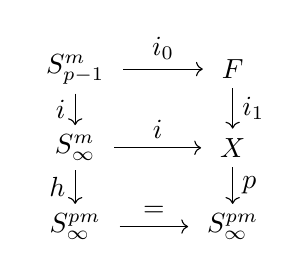
\begin{tikzpicture}[]
  \node (A) at (0,1) {$\ S^m_{p-1}\ $};
  \node (B) at (2,1) {$\ F\ $};
  \node (C) at (0,0)   {$\ S^m_\infty\ $};
  \node (D) at (2,0)   {$\ X\ $};
  \node (E) at (0,-1) {$\ S^{pm}_\infty\ $};
  \node (F) at (2,-1) {$\ S^{pm}_\infty\ $};
  \draw[->] (A) -- node[above] {$i_0$} (B);
  \draw[->] (C) -- node[above] {$i$} (D);
  % \draw[->] (C) -- node[down] {$\simeq$} (D);
  % \draw[->] (D) -- node[down] {$r$} (C);
  \draw[->] (E) -- node[above] {$=$} (F);
  \draw[->] (A) -- node[left] {$i$} (C);
  \draw[->] (B) -- node[right] {$i_1$} (D);
  \draw[->] (C) -- node[left] {$h$} (E);
  \draw[->] (D) -- node[right] {$p$} (F);
\end{tikzpicture}

\end{paracol}

\begin{paracol}{2}

\noindent
ここで, 包含 $i_0:(S^m)_{p-1}\hookrightarrow F$ が次の同型を誘導することを示す. 
\[
i_0^*:H^{*}(F;\Lambda)\ \xrightarrow{\;\cong\;}\ H^{*}\!\bigl((S^m)_{p-1};\Lambda\bigr) .
\]
$\,i_1:F\hookrightarrow X$ を包含とする. このとき $i_0^*\circ i_1^*$ は $i^*$ に同値である. 
ゆえに,
\[
i_1^*:H^{i}(X;\Lambda)\ \longrightarrow\ H^{i}(F;\Lambda)
\]
は $i<pm$ に対して単射同型である. 


% \end{paracol}

% \begin{paracol}{2}

\noindent
$G_0\subset H^{*}(F;\Lambda)$ を $i_1^*$ により $G$ に対応する部分群とする. \\
$G_0$ は $i_1^*$ の像に含まれ, $i_0^*$ は $G_0$ を,
$H^{*}\!\bigl((S^m)_{p-1};\Lambda\bigr)$ へ同型で移す. \\
injection homomorphism $i_1^*$ は, 次の写像に一致する. 
\[
H^{*}(X;\Lambda)\ \longrightarrow\ E_{\infty}^{0,*}
\longrightarrow\ E_{2}^{0,*}\ \cong\ 1\otimes H^{*}(F;\Lambda) .
\]
したがって, $r\ge2$ に対し,
\[
d_r(1\otimes G_0)=0,
\]
その極限は, $E_\infty^{*}$ において $G$ に一致する. 
また $r\ge2$ で $d_r(B^{*}\otimes 1)=0$ だから, 
\[
d_r(B^{*}\otimes G_0)=0\qquad(r\ge2).
\]
$E_\infty^{*}$ における $B^{*}\otimes G_0$ の極限を考えると, 
それは,
\[
H^{*}(X;\Lambda)\ \cong\ p^{*}H^{*}\!\bigl((S^{pm})_\infty;\Lambda\bigr)\ \otimes\ G
\]
に付随する graded module である. \\
よって, $B^{*}\otimes G_0 \cong E_\infty^{*}$ かつ,
$H^{*}(X;\Lambda)\otimes G_0$ に module として同型である. \\
これは, $B^{*}\otimes G_0$ における全ての $d_r$-像が自明であることを意味する. 

\switchcolumn

\noindent
\(i^*:H^i(S^m_\infty; \Lambda) \to H^i(S^m_{p-1}; \Lambda)\)
は, 
\(i<pm\) で同型.\\
\(G=\Lambda\gen{1, u_1,\cdots,u_{p-1}}
\subset H^*(S^m_\infty; \Lambda)\).\\
\(G=\Lambda\gen{1,r^*u_1,\cdots,r^*u_{p-1}}
\subset H^*(X; \Lambda),\ 
r^*: H^*(S^m_\infty) \cong H^*(X)\).\\
\(G_0 = \Lambda\gen{1, i_1^*r^*u_1,\cdots,i_1^*r^*u_{p-1}}
\subset H^*(F; \Lambda)\).\\
\(i_0^*=\Lambda\gen{1,i_0^*i_1^*r^*u_1,\cdots,i_0^*i_1^*r^*u_{p-1}}
= \Lambda\gen{1,u_1, \cdots,u_{p-1}}
= H^*(S^m_{p-1}; \Lambda)\).

\noindent
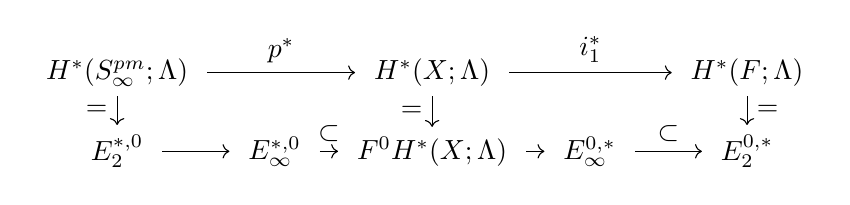
\begin{tikzpicture}[]
  \node (A) at (0,1) {$\ H^*(S^{pm}_\infty; \Lambda) \ $};
  \node (B) at (4,1) {$\ H^*(X; \Lambda)\ $};
  \node (C) at (8,1)   {$\ H^*(F; \Lambda)\ $};
  \node (D) at (0,0)   {$\ E_2^{*, 0}\ $};
  \node (E) at (2,0)   {$\ E_\infty^{*, 0}\ $};
  \node (F) at (4,0)   {$\ F^0 H^*(X; \Lambda)\ $};
  \node (G) at (6,0)   {$\ E_\infty^{0, *}\ $};
  \node (H) at (8,0)   {$\ E_2^{0, *}\ $};
  \draw[->] (A) -- node[above] {$p^*$} (B);
  \draw[->] (B) -- node[above] {$i_1^*$} (C);
  \draw[->] (A) -- node[left] {$=$} (D);
  \draw[->] (B) -- node[left] {$=$} (F);
  \draw[->] (C) -- node[right] {$=$} (H);
  \draw[->] (D) -- node[] {} (E);
  \draw[->] (E) -- node[above] {$\subset$} (F);
  \draw[->] (F) -- node[] {} (G);
  \draw[->] (G) -- node[above] {$\subset$} (H);
\end{tikzpicture}

\noindent
\(G_0\) の元は, \(E_\infty^{0,*}\) まで生き残る.

\noindent
\(d_r(x\cdot y) = d_r(x)\cdot y + (-1)^{\deg x}x\cdot d_r(y)\).

% \(r\ge2\) のとき, \(d_r\) によって, \(y\) 座標の次元が下がるので,\\
% \(d_r\ne 0\) となる可能性があるのは, 
% \(d_r(1\otimes f_0)\) の \(y\) 座標が \(G_0\) の次元に入る場合だけ.


\end{paracol}

\begin{paracol}{2}

\noindent
$G_0$ に含まれない $H^{*}(F;\Lambda)$ の最小次数の元を $f_0$ と仮定する. \\
このとき, $d_r(1\otimes f_0)$ は $B^{*}\otimes G_0$ に属するので,
\[
d_r(1\otimes f_0)=0\qquad(r\ge2).
\]
%  (次ページへ続く) 
以上より, $r\ge2$ に対し $1\otimes f_0$ は $d_r$-像ではないから, 
$1\otimes f_0\ne0$ が $E_\infty^{*}$ に残る. \\
しかし, これは $B^{*}\otimes G_0\cong E_\infty^{*}$ と矛盾する. \\
したがって, そのような $f_0$ は存在しない. ゆえに, 次が示された.
\[
H^{*}(F;\Lambda)=G_0,\qquad
i_0^{*}:H^{*}(F;\Lambda)\xrightarrow{\;\cong\;}
H^{*}\!\bigl((S^{m})_{p-1};\Lambda\bigr).
\]


\switchcolumn

\noindent
\(r\ge2\) のとき, \(d_r\) によって, \(y\) 座標の次元が下がるので,\\
\(d_r\ne 0\) となる可能性があるのは, 
\(d_r(1\otimes f_0)\) の \(y\) 座標が \(G_0\) の次元に入る場合だけ.

\end{paracol}

\begin{paracol}{2}

\noindent
一般化された Whitehead の定理 (Serre \cite{Serre1953b}) を, 
包含 $i_0:(S^m)_{p-1}\hookrightarrow F$ に適用すると, 
\[
i_{0*}:\ \pi_i\bigl((S^m)_{p-1}\bigr)\ \xrightarrow{}\ \pi_i(F)
\]
は, $m$ が奇数, かつ $p=2$ のとき同型であり, 
$m$ が偶数のとき, $p$-primary 成分の同型である. \\
対 \(((S^m)_\infty,(S^m)_{p-1})\) と \((X,F)\) に付随する
homotopy 群の完全列を, \\
homotopy 同値な包含写像 $(S^m)_\infty\hookrightarrow X$ 
により比較すると, five lemma から, 
\[
i_*:\ \pi_i\bigl((S^m)_\infty,(S^m)_{p-1}\bigr)\ \xrightarrow{\;\cong\;}\ \pi_i(X,F)
\]
は, $m$ が奇数, かつ $p=2$ のとき同型であり, 
$m$ が偶数のとき, $p$-primary 成分の同型である. \\
よって, 図式

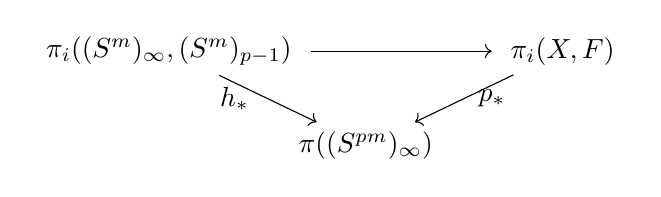
\begin{tikzpicture}[]
  \node (A) at (0,1.2) {$\ \pi_i((S^m)_\infty, (S^m)_{p-1})\ $};
  \node (B) at (5,1.2) {$\ \pi_i(X, F)\ $};
  \node (C) at (2.5,0)   {$\ \pi((S^{pm})_\infty)\ $};
  \draw[->] (A) -- node[above] {} (B);
  \draw[->] (A) -- node[left] {$h_*\,\,$} (C);
  \draw[->] (B) -- node[right] {$\,p_*$} (C);
\end{tikzpicture}

\noindent
が可換であり, $p_*$ が全ての $i$ で同型であることから, Th  \ref{thm:2.4} が従う. 
\qed

\switchcolumn

\noindent
\cite{Serre1953b}
J.-P.~Serre,
\newblock Groups d'homotopie et classes groupes abéliens,
\newblock Ann. of Math., {\bf 58} (1953), 258--294.

\noindent
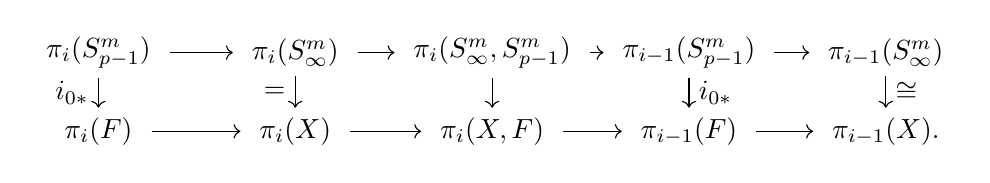
\begin{tikzpicture}[]
  \node (A) at (0,1) {$\ \pi_i(S^{m}_{p-1}) \ $};
  \node (B) at (2.5,1) {$\ \pi_i(S^m_\infty)\ $};
  \node (C) at (5,1) {$\ \pi_i(S^m_\infty, S^m_{p-1})\ $};
  \node (D) at (7.5,1) {$\ \pi_{i-1}(S^m_{p-1})\ $};
  \node (E) at (10,1) {$\ \pi_{i-1}(S^m_\infty)\ $};
  \node (F) at (0,0) {$\ \pi_i(F)\ $};
  \node (G) at (2.5,0) {$\ \pi_i(X)\ $};
  \node (H) at (5,0) {$\ \pi_i(X,F)\ $};
  \node (I) at (7.5,0) {$\ \pi_{i-1}(F)\ $};
  \node (J) at (10,0) {$\ \pi_{i-1}(X).\ $};
  \draw[->] (A) -- node[] {} (B);
  \draw[->] (B) -- node[] {} (C);
  \draw[->] (C) -- node[] {} (D);
  \draw[->] (D) -- node[] {} (E);
  \draw[->] (A) -- node[left] {$i_{0*}$} (F);
  \draw[->] (B) -- node[left] {$=$} (G);
  \draw[->] (C) -- node[] {} (H);
  \draw[->] (D) -- node[right] {$i_{0*}$} (I);
  \draw[->] (E) -- node[right] {$\cong$} (J);
  \draw[->] (F) -- node[] {} (G);
  \draw[->] (G) -- node[] {} (H);
  \draw[->] (H) -- node[] {} (I);
  \draw[->] (I) -- node[] {} (J);
\end{tikzpicture}

\end{paracol}

\begin{paracol}{2}

以上から, $m>1$ のとき写像
\[
h_m:\ \bigl((S^m)_\infty,\ S^m\bigr)\ \longrightarrow\ \bigl((S^{2m})_\infty,\ e_0\bigr)
\]
は, 上のTh の条件を満たす. したがって,
\[
h_{m*}:\ \pi_i\bigl((S^m)_\infty,\ S^m\bigr)\ \longrightarrow\ \pi_i\bigl((S^{2m})_\infty\bigr)
\]
は, $m$ が奇数なら全ての $i$ で同型, $m$ が偶数なら
2-primary 成分について全ての $i$ で同型. \\
また, $m$ が偶数で \(i<(3m-1)\) のとき同型である.

次に, 対 \(\bigl((S^m)_\infty,\ S^m\bigr)\) に対する homotopy 完全列を考える：
\begin{equation}\label{2.8}
\cdots\ \to\ \pi_i(S^m)\ \to\ \pi_i\bigl((S^m)_\infty\bigr)\ \to\
\pi_i\bigl((S^m)_\infty,\ S^m\bigr)\ \xrightarrow{\ \partial\ }\ \pi_{i-1}(S^m)\ \to\ \cdots
\tag{2.8}
\end{equation}

\end{paracol}

\begin{paracol}{2}

\noindent
準同型 \(\Delta\) を次で定義する. 
\begin{equation}\label{2.9}
\Delta\ :=\ \partial\ \circ\ (h_{m*})^{-1}\ \circ\ \Omega_1:\ 
\pi_{i+1}(S^{2m+1})\ \longrightarrow\ \pi_{i-1}(S^m)\big/\partial\Ker(h_{m*})
\tag{2.9}
\end{equation}
ここで, \(\partial\Ker(h_{m*})\) は, 
\(m\) が奇数または \(i<3m-1\) のとき自明であり, \\
\(m\) が偶数のとき有限群で, 2-torsion を含まない. \\
さらに, 準同型 \(\Delta^{-1}\) を次で定義する. 
\begin{equation}\label{2.10}
\Delta^{-1}\ :=\ \Omega_1^{-1}\ \circ\ h_{m*}\ \circ\ \partial^{-1}:\ 
\pi_{i-1}(S^m)\ \longrightarrow\ 
\pi_{i+1}(S^{2m+1})\big/ H\pi_{i+1}(S^{m+1})
\tag{2.10}
\end{equation}
を定める. ここで \(H\pi_{i+1}(S^{m+1})\) は, \(\Delta\) の kernel であることに注意する. 

%  (次ページへ続く) 

\noindent
(2.4) の可換性と, (2.7),(2.9) の $H$ と $\Delta$ の定義から, 
次の完全列を得る：
\begin{equation}\label{2.11}
% (2.11).\
\cdots\ \longrightarrow\ 
\pi_i(S^m)\xrightarrow{\,E\,}\pi_{i+1}(S^{m+1})\xrightarrow{\,H\,}
\pi_{i+1}(S^{2m+1})\xrightarrow{\,\Delta\,}\pi_{i-1}(S^m)\xrightarrow{\,E\,}\cdots
\tag{2.11}
\end{equation}
これは $m$ が奇数, あるいは $i<3m-1$ のとき成り立つ. \\
$m$ が偶数で, $i\ge 3m-1$ の場合には, \eqref{2.11} を
2-成分に関する完全列として考える. 

\begin{proposition}\label{prop:2.5}
% Prop2.5\
$\alpha\in\pi_{i+1}(S^{2m+1}), \ \beta\in \pi_{j-1}(S^{i-1})$ 対して, 
\[
\Delta\alpha\ \circ\ \beta\ \subset\ \Delta(\alpha\circ E^2\beta).
\]
特に, 任意の $\gamma$ に対し,
\[
\Delta(E^2\gamma)\ \ni\ \pm\,[\,\iota_m,\ \iota_m\,]\circ\gamma
\]
が成り立つ. ここで $[\, ,\,]$ は Whitehead product を表す. \\
上の「$\subset$」および「$\ni$」は, $m$ が奇数, 
あるいは $j<3m-1$, \\
または, 関係する元が \(2\)-primary 成分にあるときには, 
等号「$=$」に置き換えられる. 
\end{proposition}

\end{paracol}

\begin{paracol}{2}

\noindent
\textbf{Proof.}\
相対ホモトピー群 $\pi_i(X,A,x_0)$ について復習する. \\
その元は写像 $f:(CS^{i-1},S^{i-1},e_0)\to (X,A,x_0)$ で表され, \\
境界準同型 $\partial$ は $f$ を $S^{i-1}$ に制限することで与えられる. \\
相対化 $\pi_i(X, x_0, x_0)\to\pi_i(X,x_0)$ は
$f:(CS^{i-1},S^{i-1},e_0)\to(X,x_0,x_0)$ に対して, \\
合成 $f\circ p_i:(S^i,e_0)\to(X,x_0)$ を対応させて与えられる. \\
ここで, $p_i$ は (1.17) の中で, 
\(d_{i-1}\) を使って与えられた shrinking map である. \\
相対ホモトピー群の中での合成とみなすことにより, 
\(\alpha'\in\pi_i((S^m)_\infty, S^m)\)
に対して, 
\[
\partial(\alpha'\circ\partial_0^{-1}\beta) = \partial(\alpha')\circ \beta,\quad
% \]
% \[
h_{m*}(\alpha'\circ\partial_0^{-1}\beta) = h_{m*}(\alpha')\circ E\beta .
\]
また, 
\(
\partial_0:\pi_j(CS^{i-1},S^{i-1})\rightarrow \pi_{j-1}(S^{i-1})
\)
は同型である. よって,
\begin{align*}
\Delta\alpha\circ\beta
& =\partial\,(h_{m*}^{-1}\Omega_1\alpha)\circ\beta
=\partial(h_{m*}^{-1}(\Omega_1\alpha)\circ \partial_0^{-1}\beta)\\
& \subset \partial(h_{m*}^{-1}(\Omega_1(\alpha)\circ E\beta))
=\partial(h_{m*}^{-1}(\Omega_1(\alpha\circ E^2\beta)))\\
& =\Delta(\alpha\circ E^2\beta).
\end{align*}
また, $\Delta(\iota_{2m+1})$ は
\(S^m\) に \(2m\)-cell $(S^m)_2 - S^m$ を貼りつける接着写像である. 

これは, identification $(S^m\times S^m, S^m\vee S^m)\to((S^m)_2,S^m)$ の下で, \\
\(S^m\vee S^m\) 上に cell \((S^m-e_0)\times(S^m-e_0)\) を貼りつける 
接着写像の象に等しい. \\
Whitehead 積の定義から,
\(
\Delta(\iota_{2m+1})=\pm[\,\iota_m,\iota_m\,]
\)
が直ちに従い, 特に,
\[
\Delta(E^2\gamma)=\pm[\,\iota_m,\iota_m\,]\circ\gamma.\qquad \qed
\]

\switchcolumn

\noindent
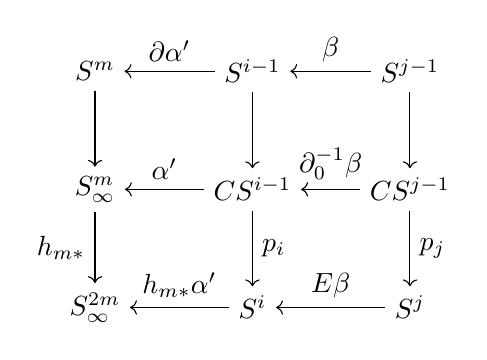
\begin{tikzpicture}[]
  \node (A) at (0,3) {$S^{m}$};
  \node (B) at (2,3) {$S^{i-1}$};
  \node (C) at (4,3) {$S^{j-1}$};
  \node (D) at (0,1.5) {$S^m_\infty$};
  \node (E) at (2,1.5) {$CS^{i-1}$};
  \node (F) at (4,1.5) {$CS^{j-1}$};
  \node (G) at (0,0) {$S^{2m}_\infty$};
  \node (H) at (2,0) {$S^i$};
  \node (I) at (4,0) {$S^j$};
  \draw[->] (B) -- node[above] {$\partial\alpha'$} (A);
  \draw[->] (C) -- node[above] {$\beta$} (B);
  \draw[->] (E) -- node[above] {$\alpha'$} (D);
  \draw[->] (F) -- node[above] {$\partial_0^{-1}\beta$} (E);
  \draw[->] (H) -- node[above] {$h_{m*}\alpha'$} (G);
  \draw[->] (I) -- node[above] {$E\beta$} (H);
  \draw[->] (A) -- node[] {} (D);
  \draw[->] (B) -- node[] {} (E);
  \draw[->] (C) -- node[] {} (F);
  \draw[->] (D) -- node[left] {$h_{m*}$} (G);
  \draw[->] (E) -- node[right] {$p_i$} (H);
  \draw[->] (F) -- node[right] {$p_j$} (I);
\end{tikzpicture}

\noindent
\(h_m:(S^m_\infty, S^m) \to (S^{2m}_\infty, e_0)\)
は, \(e^{2m}\) を \(S^{2m}-e_0\) に同相に移すので,\\
\(\psi:(CS^{2m-1}, S^{2m-1}) \to (S^m_\infty, S^m)\)
を \(2m\)-cell \(S^m_2-S^m\) の特性写像とすると,\\
\(h_m\circ\psi: (CS^{2m-1},S^{2m-1})\to(S^{2m}_\infty, e_0)\)
は, \(\Omega_1(\iota_{2m+1}) = [i] \in \pi_{2m}(S^{2m}_\infty)\)
を表す.\\
\because \
\(\Delta(\iota_{2m+1}) 
= \partial\circ h_{m*}^{-1}\circ\Omega_1(\iota_{2m+1})
= \partial[\psi] = [\psi\ |_{S^2m-1}]\).


\noindent
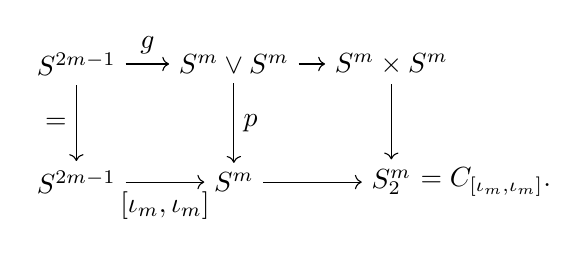
\begin{tikzpicture}[]
  \node (A) at (0,3) {$S^{2m-1}$};
  \node (B) at (2,3) {$S^{m}\vee S^{m}$};
  \node (C) at (4,3) {$S^{m}\times S^{m}$};
  \node (D) at (0,1.5) {$S^{2m-1}$};
  \node (E) at (2,1.5) {$S^{m}$};
  \node (F) at (4,1.5) {$S^{m}_2$};
  \node (G) at (5.2,1.5) {$=C_{[\iota_m, \iota_m]}.$};
  \draw[->] (A) -- node[above] {$g$} (B);
  \draw[->] (B) -- node[above] {} (C);
  \draw[->] (D) -- node[below] {$[\iota_m, \iota_m]$} (E);
  \draw[->] (E) -- node[] {} (F);
  \draw[->] (A) -- node[left] {$=$} (D);
  \draw[->] (B) -- node[right] {$p$} (E);
  \draw[->] (C) -- node[] {} (F);
\end{tikzpicture}


\end{paracol}

\begin{paracol}{2}


\begin{proposition}\label{prop:2.6}
$\alpha\in[K, S^m], \ \beta\in\pi_k(K), \ \gamma\in\pi_i(S^k)$ が,
\[
E(\alpha\circ\beta)=\beta\circ\gamma=0
\]
を満たすとする. このとき, 
\[
H\todai[1]{E\alpha,E\beta,E\gamma}\ =\ -\,\Delta^{-1}(\alpha\circ\beta)\ \circ\ E^2\gamma .
\]
\end{proposition}

\noindent
\textbf{Proof.}\
$a:(K,x_0)\to(S^m,e_0)$, $b:(S^k,e_0)\to(K,x_0)$ を
それぞれ $\alpha,\beta$ の代表とする. \\
空間 $K\cup_{b} CS^k$ を考え, 
$\overline{b}:(CS^k_x,S^k)\to(K\cup_{\beta}CS^k,\ K)$ を特性写像とする. \\
包含写像 $i:S^m\into (S^m)_\infty$ を考える. \\
(2.3),(2.4) から $E(\alpha\circ\beta)=0$ は $i_*\alpha\circ\beta=0$ を導く. \\
したがって, $a\circ b$ は $(S^m)_\infty$ で null-homotopic であり, 
$a:(K,x_0)\to(S^m,e_0)$ は,
\[
\overline{a}:\ (K\cup_{b}CS^k,\ K)\ \longrightarrow\ ((S^m)_\infty,\ S^m)
\]
へ拡張することができる. 
このとき, 下図を可換にする写像 $a'$ が存在する：
\[
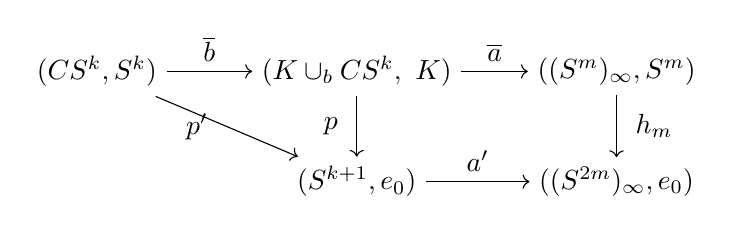
\begin{tikzpicture}[baseline=(current bounding box.center)]
  \node (A) at (0,1.4) {$(CS^k,S^k)$};
  \node (B) at (3.3,1.4) {$(K\cup_{b}CS^k,\ K)$};
  \node (C) at (6.6,1.4) {$((S^m)_\infty,S^m)$};
  \node (D) at (3.3,0)   {$(S^{k+1},e_0)$};
  \node (E) at (6.6,0)   {$((S^{2m})_\infty,e_0)$};
  \draw[->] (A)--node[above] {$\ \overline{b}\ $}(B);
  \draw[->] (B)--node[above] {$\ \overline{a}\ $}(C);
  \draw[->] (A)--node[left] {$\ p'\ $}(D);
  \draw[->] (B)--node[left] {$\ p\ $}(D);
  \draw[->] (D)--node[above] {$\ a'\ $}(E);
  \draw[->] (C)--node[right] {$\ h_m\ $}(E);
\end{tikzpicture}
\]
ここで, $p,p'$ は \(d_k\) により定義された (1.17) の shrinking map である. \\
$a\circ b$ は $\alpha\circ\beta$ を表すので, 
$\overline{a}\circ\overline{b}$ は $\partial^{-1}(\alpha\circ\beta)$ の元を表す. \\
よって, $a'\circ p'$ と $a'$ は, 
$h_{m*}\!\bigl(\partial^{-1}(\alpha\circ\beta)\bigr)$ の元を表す. \\
次に, $\gamma$ の coextension \(\coext{\gamma}\) の代表
$\widetilde{c}:S^{\ell+1}\to K\cup_{\beta}CS^k$ をを考える. \\
(1.18) より, $p\circ\widetilde{c}$ は $E\gamma$ を表す. \\
Prop 1.7 から, $\overline{a}\circ\widetilde{c}:S^{i+1}\to(S^m)_\infty$ は,
Toda bracket $\toda{i_*\alpha,\beta,\gamma}$ の元を表すので,
\[
[h_m\circ \ext{a}\circ\widetilde{c}]=[\,a'\circ p\circ\widetilde{c}\,]
\]
は, $h_{m*}\{\,i_*\alpha,\beta,\gamma\,\}$ と,
$h_{m*}\!\bigl(\partial^{-1}(\alpha\circ\beta)\bigr)\circ E\gamma$ 
の共通元である. 
\begin{align*}
H\todai[1]{E\alpha,E\beta,E\gamma}
& = H\todai[1]{\Omega_1^{-1}i_*\alpha,E\beta,E\gamma}
&& \text{by (2.4)},\\
& = -H(\Omega_1^{-1}\toda{i_*\alpha,\beta,\gamma})
&& \text{by Prop1.3},\\
& = -\Omega_1^{-1}h_{m*}\todai{i_*\alpha,\beta,\gamma} .
&& \text{by (2.7)}.\\
\Delta^{-1}(\alpha\circ\beta)\circ E^2\gamma
& = \Omega_1^{-1}h_{m*}(\partial^{-1}(\alpha\circ\beta))\circ E^2\gamma
&& \text{by (2.7)},\\
& = \Omega_1^{-1}(h_{m*}(\partial^{-1}(\alpha\circ\beta))\circ E\gamma).
&& \text{by (1.12)}.
\end{align*}

\switchcolumn

\noindent
\(S^m\xleftarrow{\alpha}
K\xleftarrow{\beta}
S^k \xleftarrow{\gamma} S^i\).

\noindent
\textbf{(2.3).}\
\(\Omega_1 = i_*^{-1}\circ\Omega_0:
[EK, S^{m+1}]\xrightarrow{\cong}[K, S^m_\infty]\).

\noindent
\textbf{(2.4).}\\
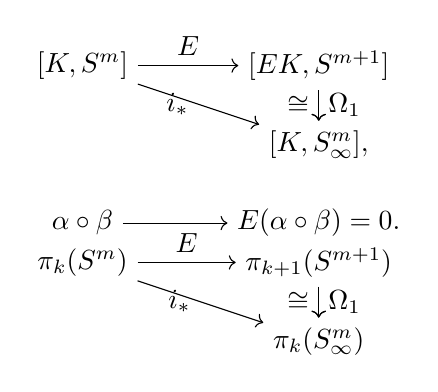
\begin{tikzpicture}[baseline=(current bounding box.center)]
  \node (A) at (0,4) {$[K, S^m]$};
  \node (B) at (3,4) {$[EK, S^{m+1}]$};
  \node (C) at (3,3) {$[K, S^m_\infty],$};
  \node (D) at (0,1.5) {$\pi_k(S^m)$};
  \node (E) at (3,1.5) {$\pi_{k+1}(S^{m+1})$};
  \node (F) at (3,0.5) {$\pi_{k}(S^{m}_\infty)$};
  \node (G) at (0,2) {$\alpha\circ\beta$};
  \node (H) at (3,2) {$E(\alpha\circ\beta)=0.$};
  \draw[->] (A)--node[above] {$E$}(B);
  \draw[->] (B)--node[right] {$\Omega_1$}(C);
  \draw[->] (B)--node[left] {$\cong$}(C);
  \draw[->] (A)--node[left] {$i_*$}(C);
  \draw[->] (D)--node[above] {$E$}(E);
  \draw[->] (E)--node[right] {$\Omega_1$}(F);
  \draw[->] (E)--node[left] {$\cong$}(F);
  \draw[->] (D)--node[left] {$i_*$}(F);
  \draw[->] (G)--node[] {}(H);
\end{tikzpicture}

\noindent
\(\overline{a}\circ\overline{b}\ |_{S^n} = a\circ b,\qquad
\partial:\pi_{k+1}(S^m_\infty, S^m)\to\pi_k(S^m)\).\\
\(h_{m*}:\pi_{k+1}(S^m_\infty,S^m)\to\pi_{k+1}(S^{2m}_\infty)\).\\
\(S^m_\infty\xleftarrow{i}
S^m\xleftarrow{\alpha}
K\xleftarrow{\beta}
S^k \xleftarrow{\gamma}
S^j,\qquad
i_*\alpha\circ\beta=0,\ 
\beta\circ\gamma=0.\)

\noindent
\textbf{(1.18).}\
\(p_*(\widetilde{\delta}) = E\delta,\qquad
\widetilde{\delta}\in[EV, X\cup_\gamma CW]:\
\delta\in [V,W]\) の coextension.

\noindent
\textbf{Prop1.7.}\
\((-1)^n\todai[n]{\alpha, E^n\beta, E^n\gamma}
= \gen{\overline{\alpha}\circ E^n\widetilde{\gamma}}\).\\

\noindent
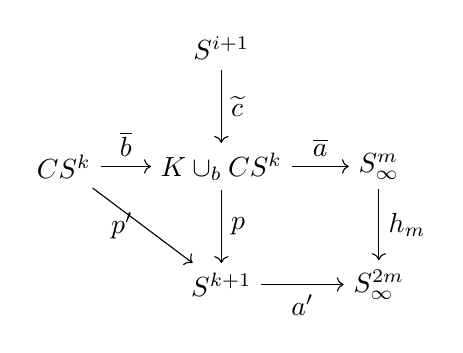
\begin{tikzpicture}[baseline=(current bounding box.center)]
  \node (A) at (2,3) {$S^{i+1}$};
  \node (B) at (0,1.5) {$CS^k$};
  \node (C) at (2,1.5) {$K\cup_b CS^k$};
  \node (D) at (4,1.5) {$S^m_\infty$};
  \node (E) at (2,0) {$S^{k+1}$};
  \node (F) at (4,0) {$S^{2m}_\infty$};
  \draw[->] (A)--node[right] {$\widetilde{c}$}(C);
  \draw[->] (B)--node[above] {$\overline{b}$}(C);
  \draw[->] (B)--node[left] {$p'$}(E);
  \draw[->] (C)--node[above] {$\overline{a}$}(D);
  \draw[->] (C)--node[right] {$p$}(E);
  \draw[->] (D)--node[right] {$h_m$}(F);
  \draw[->] (E)--node[below] {$a'$}(F);
\end{tikzpicture}

\noindent
\([h_m\circ\overline{a}\circ\widetilde{c}]
= [a'\circ p\circ\widetilde{c}]
= [a'\circ Ec]
= h_{m*}([\overline{a}\circ\overline{b}])\circ E\gamma
= h_{m*}(\partial^{-1}(\alpha\circ\beta))\circ E\gamma\).

\noindent
\textbf{(2.4).}\
\(i_* = \Omega_1\circ E:
[K, S^m]\xrightarrow{E}
[EK, S^{m+1}]\xrightarrow{\Omega_1}
[EK, S^m_\infty]\).

\noindent
\textbf{Prop1.3.}\
\(-\Omega_0\todai[m+1]{\alpha, E^{n+1}\beta, E^{n+1}\gamma}
= \todai[n]{\Omega_0\alpha, E^n\beta, E^n\gamma}\).

\noindent
\textbf{(2.7).}\
\(H = \Omega_1^{-1}\circ h_{m*}\circ\Omega_1: 
[EK, S^{m+1}]\to[EK, S^2m+1]\).

\noindent
\textbf{(2.10).}\
\(\Delta^{-1}= \Omega_1^{-1}\circ h_{m*}\circ\partial^{-1}:
\pis{i-1}{S^m}\to\pis{i+1}{S^{2m+1}}/H \pis{i+1}{S^m+1}\).

\noindent
\textbf{(1.12).}\
\(\Omega_0(\beta\circ E\alpha) = \Omega_0\beta\circ\alpha\).
  
\end{paracol}

\begin{paracol}{2}

これにより, 
\(H\todai[1]{E\alpha, E\beta, E\gamma}\) と
\(-\Delta^{-1}(\alpha\circ\beta)\circ E^2\gamma\) は, \\
共通元 $\Omega_1^{-1}[a'\circ p\circ\widetilde{c}\,]$ を持つことが分かる. \\
また, これら2つの集合は, どちらも同じ次の部分群の coset である.
\begin{align*}
& H(E\alpha\circ E\pi_{i+1}(K) + \pi_{j+1}(S^{m+1})\circ E^2\gamma)\\
& = H(E\alpha)\circ E\pi_{i+1}(K) + H\pi_{j+1}(S^{m+1})\circ E^2\gamma
&& \text{Prop2.2,}\\
& = H\pi_{j+1}(S^{m+1})\circ E^2\gamma .
&& \text{by (2.11).}
\end{align*}
以上より, 
\[
H\todai[1]{E\alpha,E\beta,E\gamma}\ 
=\ -\,\Delta^{-1}(\alpha\circ\beta)\circ E^2\gamma
\]
が成り立つ. 
\qed

最後に, よく知られている事実として, $n$ が偶数のとき, 
\[
H[\,\iota_n,\ \iota_n\,]\ =\ \pm\,2\,\iota_{2n-1}
\]
が成り立つ. これとProp \ref{prop:2.5} から直ちに次が成り立つ. 

\begin{proposition}\label{prop:2.7}
% Prop2.7.\
$n$ が偶数のとき,
\[
H\!\bigl(\Delta(\iota_{2n+1})\bigr)\ =\ \pm\,2\,\iota_{2n-1}
\qquad (\text{cf.} (11.14)).
\]
\end{proposition}


\switchcolumn

\noindent
\textbf{Prop2.2.}\
\(H(\alpha\circ E\beta) = H(\alpha)\circ E\beta.\)

\noindent
\textbf{(2.11).}\
\(\cdots\to\pis{i}{S^m}
\xrightarrow{E}\pis{i+1}{S^{m+1}}
\xrightarrow{H}\pis{i+1}{S^{2m+1}}
\xrightarrow{\Delta}\pis{i-1}{S^m}
\to\cdots,\)\\
は, \(m:\) odd, または, \(i<3m-1\) で完全.\\

\noindent
\textbf{[西田:ホモトピー論] Th6.3.11.}\\
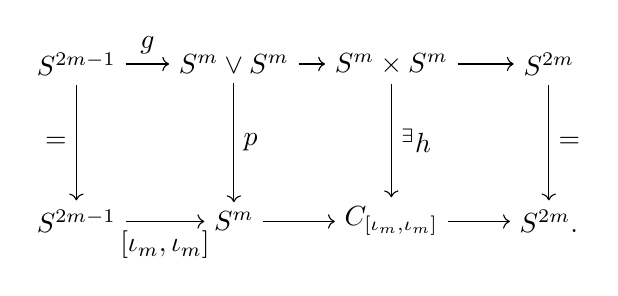
\begin{tikzpicture}[baseline=(current bounding box.center)]
  \node (A) at (0,2) {$S^{2m-1}$};
  \node (B) at (2,2) {$S^{m}\vee S^{m}$};
  \node (C) at (4,2) {$S^m\times S^m$};
  \node (D) at (6,2) {$S^{2m}$};
  \node (E) at (0,0) {$S^{2m-1}$};
  \node (F) at (2,0) {$S^{m}$};
  \node (G) at (4,0) {$C_{[\iota_m, \iota_m]}$};
  \node (H) at (6,0) {$S^{2m}.$};
  \draw[->] (A)--node[above] {$g$}(B);
  \draw[->] (A)--node[left] {$=$}(E);
  \draw[->] (B)--node[] {}(C);
  \draw[->] (B)--node[right] {$p$}(F);
  \draw[->] (C)--node[] {}(D);
  \draw[->] (C)--node[right] {${}^{\exists}h$}(G);
  \draw[->] (D)--node[right] {$=$}(H);
  \draw[->] (E)--node[below] {$[\iota_m, \iota_m]$}(F);
  \draw[->] (F)--node[] {}(G);
  \draw[->] (G)--node[] {}(H);
\end{tikzpicture}

\noindent
\(H^m(S^m\times S^m) = \z\gen{u_1}\oplus\z\gen{u_2}\)
とすると,
\(H^{2m}(S^m\times S^m) = \z\gen{u_1 u_2},
u_1^2 = u_2^2 = 0 .\)\\
\(H^n(C_{[\iota_n, \iota_n]}) = \z\gen{\overline{u}},\
H^{2n}(C_{[\iota_n, \iota_n]}) = \z\gen{\overline{v}}\)
とすると, \\
\(h^*(\overline{u}) = u_1 + u_2.\)\\
\(n:\) even のとき, \(u_1 u_2 = u_2 u_1\) なので,
(\(n\):odd のとき, \(u_1 u_2 = - u_2 u_1\) ).\\
\(h^*(\overline{u}^2) = (u_1 + u_2)^2
= u_1^2 + u_1 u_2 + u_2 u_1 + u_2^2 = 2u_1 u_2.\)\\
\(h^*:H^{2n}(C_{[\iota_n, \iota_n]})\to H^{2n}(S^n\times S^n)\)
は, 同型なので,
\(\overline{u}^2 = 2\overline{v}\).\\
Hopf invariant の定義により, 
\(H[\iota_n, \iota_n] = \pm2.\)


\end{paracol}

\begin{paracol}{2}



\newpage

\renewcommand{\refname}{References}
\begin{thebibliography}{99}

\bibitem{Adams1960}
J.~F.~Adams,
\newblock On the non-existence of elements of Hopf invariant one,
\newblock Ann. of Math., {\bf 72} (1960), 20--104.

\bibitem{Adem}
J.~Adem,
\newblock The relations on Steenrod powers of cohomology classes,
\newblock Algebraic geometry and topology, Princeton.

\bibitem{Barratt1955}
M.~G.~Barratt,
\newblock Track groups I, II,
\newblock Proc. London Math. Soc., {\bf 5} (1955), 71--106, 285--329.

\bibitem{Barratt1961}
M.~G.~Barratt,
\newblock Note on a formula due to Toda,
\newblock Jour. London Math. Soc., {\bf 36} (1961), 95--96.

\bibitem{BarrattHilton1953}
M.~G.~Barratt and P.~J.~Hilton,
\newblock On join operations of homotopy groups,
\newblock Proc. London Math. Soc., {\bf 3} (1953), 430--445.

\bibitem{BlakersMassey1952}
A.~L.~Blakers and W.~S.~Massey,
\newblock The homotopy groups of a triad II,
\newblock Ann. of Math., {\bf 55} (1952), 192--201.

\bibitem{Freudenthal1937}
H.~Freudenthal,
\newblock Über die Klassen der Sphärenabbildungen,
\newblock Compos. Math., {\bf 5} (1937).

\bibitem{Hopf1935}
H.~Hopf,
\newblock Über die Abbildungen von Sphären auf Sphären niedriger Dimension,
\newblock Fund. Math., {\bf 25} (1935).

\bibitem{James1955}
I.~M.~James,
\newblock Reduced product spaces,
\newblock Ann. of Math., {\bf 62} (1955), 170--197.

\bibitem{James1956}
I.~M.~James,
\newblock Suspension triad of a sphere,
\newblock Ann. of Math., {\bf 63} (1956), 407--429.

\bibitem{James1958}
I.~M.~James,
\newblock The intrinsic join: A study of the homotopy groups of Stiefel manifold,
\newblock Proc. London Math. Soc., {\bf 8} (1958), 507--535.

\bibitem{Moore1953}
J.~C.~Moore,
\newblock Some applications of homology theory to homotopy problems,
\newblock Ann. of Math., {\bf 58} (1953), 325--350.

\bibitem{Serre1951}
J.-P.~Serre,
\newblock Homologie singulière des espaces fibrés,
\newblock Ann. of Math., {\bf 54} (1951), 425--505.

\bibitem{Serre1953a}
J.-P.~Serre,
\newblock Cohomologie modulo 2 des complexes d'Eilenberg-MacLane,
\newblock Comm. Math. Helv., {\bf 27} (1953), 198--231.

\bibitem{Serre1953b}
J.-P.~Serre,
\newblock Groups d'homotopie et classes groupes abéliens,
\newblock Ann. of Math., {\bf 58} (1953), 258--294.

\bibitem{Serre1953c}
J.-P.~Serre,
\newblock Quelques calculs de groupes d'homotopie,
\newblock Comptes Rendus Paris, {\bf 236} (1953), 2475--2477.

\bibitem{Steenrod1951}
N.~E.~Steenrod,
\newblock Topology of fibre bundles,
\newblock Princeton.

\bibitem{Steenrod1949}
N.~E.~Steenrod,
\newblock Cohomology invariants of mappings,
\newblock Ann. of Math., {\bf 50} (1949), 954--988.

\bibitem{Steenrod1953}
N.~E.~Steenrod,
\newblock Cyclic reduced powers of cohomology classes,
\newblock Proc. Nat. Acad. Sci. U.S.A., {\bf 39} (1953), 217--223.

\bibitem{Toda1952}
H.~Toda,
\newblock Generalized Whitehead products and homotopy groups of spheres,
\newblock Jour. of Inst. Poly. Osaka City Univ., {\bf 3} (1952), 43--82.

\bibitem{Toda1956}
H.~Toda,
\newblock On double suspension $E^2$,
\newblock Jour. of Inst. Poly. Osaka City Univ., {\bf 7} (1956), 103--145.

\bibitem{Toda1957}
H.~Toda,
\newblock Reduced join and Whitehead product,
\newblock Jour. of Inst. Poly. Osaka City Univ., {\bf 8} (1957), 15--30.

\bibitem{Toda1958a}
H.~Toda,
\newblock On exact sequences in Steenrod algebra mod 2,
\newblock Memoirs Univ. of Kyoto, {\bf 31} (1958), 33--64.

\bibitem{Toda1958b}
H.~Toda,
\newblock $p$-primary components of homotopy groups II. mod $p$ Hopf invariant,
\newblock Memoirs Univ. of Kyoto, {\bf 31} (1958), 143--160.

\bibitem{Toda1959}
H.~Toda,
\newblock $p$-primary components of homotopy groups IV. Compositions and toric constructions,
\newblock Memoirs Univ. of Kyoto, {\bf 32} (1959), 297--332.

\bibitem{Whitehead1950a}
G.~W.~Whitehead,
\newblock A generalization of the Hopf invariant,
\newblock Ann. of Math., {\bf 51} (1950), 192--237.

\bibitem{Whitehead1950b}
G.~W.~Whitehead,
\newblock The $(n+2)$nd homotopy group of the $n$-sphere,
\newblock Ann. of Math., {\bf 52} (1950), 245--247.

\bibitem{Whitehead1941}
J.~H.~C.~Whitehead,
\newblock On adding relations to homotopy groups,
\newblock Ann. of Math., {\bf 42} (1941), 409--428.

\bibitem{Whitehead1944}
J.~H.~C.~Whitehead,
\newblock On the groups $\pi_n(V_{m,n})$ and sphere bundles,
\newblock Proc. London Math. Soc., {\bf 48} (1944), 243--291.

\end{thebibliography}



\end{paracol}

\end{document}
